\section{Topic}
\label{sec:topic}



\subsection{Notation}
Throughout this Chapter the following notation is used:
\begin{itemize}
    \item $ \phi $ is a conjunction of DL constraints.
    It is being checked for SAT.
    \item $ x - y \prec c $ is a general form
    of a DL constraint in $ \phi $ where $ \prec \; \in \{ <, \leq \} $.
    \item $ \mathbb{D} $ is a domain over which
    the variables and constants in $ \phi $ are defined
    (\eg $ \mathbb{R} $).
\end{itemize}



\subsection{Constraint Graph}
\begin{figure}[htb]
    \begin{center}
        \begin{tabular}{cc}
            \begin{minipage}{0.45\linewidth}
                \begin{center}
                    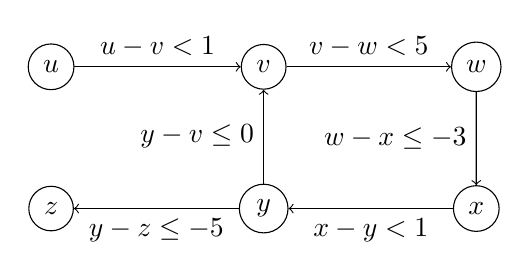
\begin{tikzpicture}[scale=0.9,state/.style={draw, circle, fill=none,text centered, text=black}]
    \node[state] (u) at (0, 2) {$u$};
    \node[state] (v) at (3, 2) {$v$};
    \node[state] (w) at (6, 2) {$w$};
    \node[state] (x) at (6, 0) {$x$};
    \node[state] (y) at (3, 0) {$y$};
    \node[state] (z) at (0, 0) {$z$};
    \draw [->] (u) -- node[anchor=south] {$ u-v < 1 $} (v);
    \draw [->] (v) -- node[anchor=south] {$ v-w < 5 $} (w);
    \draw [->] (w) -- node[anchor=east] {$ w-x \leq -3 $} (x);
    \draw [->] (x) -- node[anchor=north] {$ x-y < 1 $} (y);
    \draw [->] (y) -- node[anchor=north] {$ y-z \leq -5 $} (z);
    \draw [->] (y) -- node[anchor=east] {$ y-v \leq 0 $} (v);
\end{tikzpicture}

                \end{center}
            \end{minipage}
            &
            \begin{minipage}{0.45\linewidth}
                \begin{center}
                    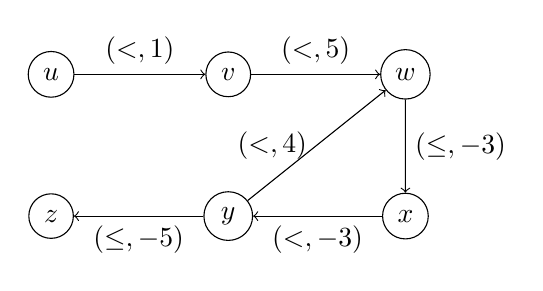
\begin{tikzpicture}[scale=0.9,state/.style={draw, circle, fill=none,text centered, text=black}]
    \node[state] (u) at (0, 2) {$u$};
    \node[state] (v) at (2.5, 2) {$v$};
    \node[state] (w) at (5, 2) {$w$};
    \node[state] (x) at (5, 0) {$x$};
    \node[state] (y) at (2.5, 0) {$y$};
    \node[state] (z) at (0, 0) {$z$};
    \draw [->] (u) -- node[anchor=south] {$ (<,1) $} (v);
    \draw [->] (v) -- node[anchor=south] {$ (<,5) $} (w);
    \draw [->] (w) -- node[anchor=west] {$ (\leq,-3) $} (x);
    \draw [->] (x) -- node[anchor=north] {$ (<,-3) $} (y);
    \draw [->] (y) -- node[anchor=north] {$ (\leq,-5) $} (z);
    \draw [->] (y) -- node[anchor=east] {$ (<,4) $} (w);
\end{tikzpicture}

                \end{center}
            \end{minipage}
        \end{tabular}
    \end{center}
    \caption{Examples of constraint graphs for
        Equation~\ref{eq:example-2} (left) and
        Equation~\ref{eq:example-3} (right).}
    \label{fig:contraints-graphs}
\end{figure}
Constraint graph (Figure~\ref{fig:contraints-graphs})
is a weighted directed graph which represents $ \phi $
and which is used by a DL constraints checker
(Figure~\ref{fig:lazy-and-incremental-approaches}) to test
if $ \phi $ is SAT.
In~\cite{cotton2004some} it is defined as follows:
\begin{definition}[Constraint Graph]
    \label{def:constraint-graph}
    The constraint graph is a graph $ \Gamma = (V,E,weight,op) $ where:
    \begin{itemize}
        \item $ V $ is a set of vertices. Each vertex $ x \in V $
        corresponds to one numeric variable occurring in $ x - y \prec c $.
        \item $ E $ is a set of directed edges. Each edge
        $ (x,y) \in E $ corresponds to $ x - y \prec c $.
        \item $ weight: E \mapsto \mathbb{D} $ is a weight function.
        It maps each edge $ (x,y) \in E $ to the constant
        $ c \in \mathbb{D} $ from the corresponding DL inequality
        $ x - y \prec c $.
        \item $ op: E \mapsto \{ <, \leq \} $ is a function which
        maps each edge $ (x,y) \in E $ to the operation
        $ \prec $ from the corresponding DL inequality
        $ x - y \prec c $.
    \end{itemize}
\end{definition}




\subsection{Negative Cycles in Constraint Graph}
There is a direct correspondence between a negative cycle
in a constraint graph and SAT of $ \phi $ represented by this graph.

A path in the graph corresponds to a sum of the corresponding
constraints. \Eg the path
$ u \rightarrow v \rightarrow w \rightarrow x $
in the left graph on Figure~\ref{fig:contraints-graphs}
corresponds to the following sum of the DL inequalities:
\begin{equation}
    \begin{aligned}
        u - v & < \;\;\; 1 \\
        v - w & < \;\;\; 5 \\
        w - x & \leq -3 \\
        \hline
        u - x & < \;\;\; 3
    \end{aligned}
\end{equation}
If at least one strict inequality is present
then the resulting inequality will also be strict.
This summation along a path can also be expressed with
an inferred transitivity constraint
(\eg~Equation~\ref{eq:transitivity-example}).
The transitivity constraint naturally follows from $ \phi $ and
therefore must be satisfied in order to satisfy $ \phi $.

A cycle in the constraint graph corresponds to an inequality
$ 0 \prec c $
which may cause a conflict in the following situations:
\begin{itemize}
    \item $ c < 0$
    \item $ c = 0 $ and $ \prec $ is $ < $
    (can be checked with $ op $ from Definition~\ref{def:constraint-graph})
\end{itemize}

An example of a conflict can be seen on the right graph
on Figure~\ref{fig:contraints-graphs}.
The conflict corresponds to the negative cycle
$ x \rightarrow y \rightarrow w \rightarrow x $
which corresponds to the following conflicting inequalities:
\begin{equation}
    \begin{aligned}
        x - y & < -3 \\
        y - w & < \;\;\; 4 \\
        w - x & \leq -3 \\
        \hline
        0 & < -2
    \end{aligned}
\end{equation}



\subsection{Bellman-Ford Algorithm for Constraint Graph}
\cite{cotton2004some} uses a Goldberg-Radzik~\cite{goldberg1993heuristic}
variant of the Bellman-Ford algorithm
(Algorithm~\ref{alg:goldberg-radzik}) to detect negative cycles.
\cite{goldberg1993heuristic}~states that the algorithm has the same
worst-case complexity $ O(|V| \cdot |E|) $
as Bellman-Ford algorithm but is superior in practice.
Important terminology and notation used in the algorithm are given below:
\begin{itemize}
    \item The source vertex $ s \in V $ is a vertex from which
    the shortest paths to other vertices are computed.
    \item $ d(v) \in \mathbb{D} $ is a distance estimate
    from the source vertex to the given vertex $ v \in V $.
%    \item $ \pi(v) \in V $ is a parent of $ v \in V $ in a tree
%    of shortest paths. The tree has the source vertex as its root.
    \item $ r_d(x,y) = weight(x,y) + d(x) - d(y) $ is
    the reduced cost function~\cite{goldberg1993heuristic}.
    It shows if it is possible to improve the distance estimate $ d(y) $
    by taking a path through the intermediate vertex $ x \in V $.
    \item $ status(v) = \{ unreached, labeled, scanned \} $
    is a status of a vertex $ v \in V $.
    $ status(v) = unreached $ means $ v $ has not been explored yet.
    $ status(v) = labeled $ means $ v $ has been explored \ie
    the distance estimate for it has been updated at least once
    and potentially it can be used to improve distance estimates to
    other vertices.
    $ status(v) = scanned $ means $ v $ has been completely explored
    and will not be considered further for improving distance estimates.
    \item Edge $ (x,y) \in E $ is called admissible if $ r_d(x,y) < 0 $
    \ie this edge can improve the current distance estimate for
    the vertex $ y \in V $.
    \item Admissible graph $ \Gamma_d $ is a subgraph
    of $ \Gamma $ composed of the admissible edges of $ \Gamma $.
    It is dynamic because it depends on the distance estimates
    which may change at each iteration of
    the Algorithm~\ref{alg:goldberg-radzik}.
\end{itemize}
\begin{Algorithm}
    \caption{An algorithm for checking if $ \phi $ which corresponds
        to the input constraint graph $ \Gamma = (V,E,weight,op) $ is SAT.
        It returns SAT or UNSAT status and a set of DL constraints
        corresponding to a conflict (in case of UNSAT).
        It is based on Bellman-Ford
        algorithm~\cite[p.561]{cormen2009introduction}.
        Goldberg-Radzik heuristic~\cite{goldberg1993heuristic},
        which is used here,
        suggests to scan a graph in a topological order.
        This algorithm uses
        depth first search~\cite[p.603]{cormen2009introduction} (DFS)
        and breadth first search~\cite[p.594]{cormen2009introduction} (BFS)
        for auxiliary tasks.}
    \label{alg:goldberg-radzik}
    \begin{algorithm}{Goldberg-Radzik}
        {\text{constraint graph} \Gamma = (V,E,weight,op),
            \text{source vertex} s \in V}
        \begin{FOR}{\mathrm{each \; vertex} \; x \in V}
            d(x) = \infty \\
            status(x) = unreached
        \end{FOR} \\
        d(s) = 0 \\
        status(s) = labeled \\
        A \= \varnothing \\
        B \= \{ s \} \\
        \begin{REPEAT} \\
            \begin{IF}{\Gamma_d \text{has a cycle (DFS on} \Gamma_d \text{can be used to check it)}}
                \RETURN (UNSAT, \text{DL constraints corresponding to the detected cycle})
            \end{IF} \\
            \begin{FOR}{\mathrm{each \; vertex} \; x \in B}
                \begin{IF}{x \text{has no outgoing admissible edges}}
                    B \= B \setminus \{ x \} \\
                    status(x) = scanned
                \end{IF}
            \end{FOR} \\
            A \= \text{set of unexplored vertices reachable from}
                    B \text{in} \Gamma_d
                    \text{(BFS on} \Gamma_d \text{can be used here)} \\
            A \= \text{sort} A \text{topologically using}
                    \Gamma_d \text{as an input graph}
                    \text{(DFS on} \Gamma_d \text{can be used here)} \\
            B \= \varnothing \\
            \begin{FOR}{\mathrm{each \; vertex} \; x \in A}
                status(x) = labeled \\
                \begin{FOR}{\mathrm{each \; edge} \; (x,y) \in E}
                    \begin{IF}{d(x) + weight(x,y) < d(y)}
                        d(y) \= d(x) + weight(x,y) \\
                        \begin{IF}{status(y) = unreached}
                            B \= B \cup \{ y \}
                        \end{IF} \\
                        status(y) \= labeled \\
                        status(x) \= scanned
                    \end{IF}
                \end{FOR}
            \end{FOR}
        \end{REPEAT} A \; is \; empty \\
        \RETURN (SAT, \varnothing) \\
    \end{algorithm}
\end{Algorithm}
Some notes to the Algorithm~\ref{alg:goldberg-radzik}:
\begin{itemize}
    \item In practice, checking $ \Gamma_d $ for a cycle (line~9) and
    computing a set of vertices reachable from $ B $ (line~15) can be
    done by only one DFS call.
    However, it is two logically distinct steps and therefore they
    are performed separately in the algorithm.
    \item Unexplored vertices (line~15) are vertices which have
    status $ unreached $ \ie they have not been processed yet at that
    particular step.
    \item If $ B $ is empty or no unexplored vertices
    are reachable from it (line~15) then $ A $ will be assigned an
    empty set.
\end{itemize}

The admissible graph $ \Gamma_d $ describes a set of possible path
updates that can be used to improve distance estimates.
If it contains a cycle then it means that one can
update distance estimates infinitely by looping along
this cycle.
The idea of the Algorithm~\ref{alg:goldberg-radzik} is to det
\begin{theorem}[Name of the theorem]
    \label{the:nameOfTheorem}
    This is how you write a theorem. Do not forget to prove the theorem.
    \begin{proof}
        Here you write the proof of the theorem.
    \end{proof}
\end{theorem}



\subsection{Implementation Details}
Some implementation details (Numeric Conflict Analysis,
Reducing Feasibility Checks).



\subsection{Experimental Results}
Tell a reader about some experimental results.
